%%%%%%%%%%%%%%%%%%%%%%%%%%%%%%%%%%%%%%%%%
% University Assignment Title Page 
% LaTeX Template
% Version 1.0 (27/12/12)
%
% This template has been downloaded from:
% http://www.LaTeXTemplates.com
%
% Original author:
% WikiBooks (http://en.wikibooks.org/wiki/LaTeX/Title_Creation)
%
% License:
% CC BY-NC-SA 3.0 (http://creativecommons.org/licenses/by-nc-sa/3.0/)
% 
% Instructions for using this template:
% This title page is capable of being compiled as is. This is not useful for 
% including it in another document. To do this, you have two options: 
%
% 1) Copy/paste everything between \begin{document} and \end{document} 
% starting at \begin{titlepage} and paste this into another LaTeX file where you 
% want your title page.
% OR
% 2) Remove everything outside the \begin{titlepage} and \end{titlepage} and 
% move this file to the same directory as the LaTeX file you wish to add it to. 
% Then add \input{./title_page_1.tex} to your LaTeX file where you want your
% title page.
%
%%%%%%%%%%%%%%%%%%%%%%%%%%%%%%%%%%%%%%%%%
%\title{Title page with logo}
%----------------------------------------------------------------------------------------
%   PACKAGES AND OTHER DOCUMENT CONFIGURATIONS
%----------------------------------------------------------------------------------------

\documentclass[12pt]{report}
\usepackage[english]{babel}
\usepackage[utf8x]{inputenc}
\usepackage{amsmath}
\usepackage{graphicx}
\usepackage[colorinlistoftodos]{todonotes}
\usepackage{float}
\usepackage{hyperref}
\begin{document}

\begin{titlepage}

\newcommand{\HRule}{\rule{\linewidth}{0.2mm}} % Defines a new command for the horizontal lines, change thickness here

\center % Center everything on the page
 
%----------------------------------------------------------------------------------------
%   HEADING SECTIONS
%----------------------------------------------------------------------------------------

%\textsc{\LARGE EURECOM}\\[1.5cm] % Name of your university/college
\textsc{\Large Semester Project Report}\\[0.5cm] % Major heading such as course name
\textsc{\large Department Of Data Science and Engineering}\\[0.5cm] % Minor heading such as course title

%----------------------------------------------------------------------------------------
%   TITLE SECTION
%----------------------------------------------------------------------------------------

\HRule \\[0.4cm]
{ \Large \bfseries Emotion Patterns in Music Playlists}\\[0.4cm] % Title of your document
\HRule \\[6cm]
 
%----------------------------------------------------------------------------------------
%   AUTHOR SECTION
%----------------------------------------------------------------------------------------

\begin{minipage}{0.4\textwidth}
\begin{flushleft} \large
\emph{Authors:}\\
Sara \textsc{Giammusso} \\ Mario \textsc{Guerriero} % Your name
\end{flushleft}
\end{minipage}
~
\begin{minipage}{0.4\textwidth}
\begin{flushright} \large
\emph{Supervisors:} \\
Raphael \textsc{Troncy}\\ Pasquale \textsc{Lisena}\\ Enrico \textsc{Palumbo} % Supervisor's Name
\end{flushright}
\end{minipage}\\[2cm]

% If you don't want a supervisor, uncomment the two lines below and remove the section above
%\Large \emph{Author:}\\
%John \textsc{Smith}\\[3cm] % Your name

%----------------------------------------------------------------------------------------
%   DATE SECTION
%----------------------------------------------------------------------------------------

{\large \today}\\[2cm] % Date, change the \today to a set date if you want to be precise

%----------------------------------------------------------------------------------------
%   LOGO SECTION
%----------------------------------------------------------------------------------------


\includegraphics[width=0.3\textwidth]{logo.png}\\[1cm] % Include a department/university logo - this will require the graphicx package
 
%----------------------------------------------------------------------------------------

\vfill % Fill the rest of the page with whitespace

\end{titlepage}

\tableofcontents


\begin{abstract}

Music streaming services such as Spotify are revolutionizing the music world, enabling a transition from artist-created bundles of songs (CDs) to user-created playlists.\par
Different logics may be applied in the generation of a playlist: they can contain songs of a similar genre (e.g. ``Rock playlist''), fit to a particular occasion (e.g. ``New year's eve party''), to a particular context (e.g. ``Gym''), to a particular mood (e.g.``Happy'') and so on.\par

The goal of this semester project is to unravel the emotion patterns underlying the sequences of songs in a playlist using automatic approaches of Emotion Detection on the lyrics.

\end{abstract}
\newpage

% CHAPTER 1 - INTRODUCTION
\chapter{Introduction}
\section{Background}
In the last few years the online music streaming services such as Spotify, Apple Music and Deezer introduced, among others,  the possibility to create playlists thus opening new challenges on music recommendation.\par
One of the new possible tasks a modern Recommender System should perform is automatic playlist continuation. By suggesting appropriate songs to add to a playlist, a Recommender System can increase user engagement by making playlist creation easier, as well as extending listening beyond the end of existing playlists. \par
More precisely the task of automatic playlist continuation consists in: given a set of playlist features, the system shall generate a list of recommended tracks that can be added to that playlist, thereby ``continuing'' the playlist. \par

In fact, one of the final goals of this project was to produce numerical features to be used in a recommender system for music playlists. Specifically, this recommender system had to be built for the RecSys Challenge 2018\footnote{\url{https://recsys-challenge.spotify.com/}}, hosted for this year by Spotify, which provided a huge dataset of a milion playlist coming from their own platform. Since the goal of this challenge is to improve the playlist continuation feature of the Spotify's recommender system, we believed that putting emotions in the features used to group playlists could be useful for achieving better performances. For this reason, the output of this system is a vector where, each element, expresses the likelihood score for the releated emotion. The details of how this vector is built will be made clearer throughout this report.

\section{Project scope}

One of the possible features to consider in developing a system for the automatic playlist continuation task is the emotion expressed in each song of the playlist and the more frequent transition patterns from one emotion to the other. Thus, not only the emotion of each song lyrics must be detected, but also the transitions between emotions must be analyzed. \par
Emotion Detection is a novel and promising field of study of Natural Language Understanding, which is able to automatically infer what are the emotions expressed in a text. It can be considered as a Sentiment Analysis task, which is the computational treatment of opinions, sentiments and subjectivity of a natural language text. \par

\section{Results}

Below we just reported the accuracy results we obtained throughout our project while classifying emotions both in song lyrics and in playlists, as shown in table \ref{tab:compar} and \ref{tab:compar2} respectively.

\begin{table}[H]
\centering
\begin{tabular}{ |p{3cm}||p{1.5cm}|p{1.5cm}|p{1.5cm}|p{1.5cm}|  }
 \hline
 \multicolumn{5}{|c|}{10-fold Cross Validation Accuracy} \\
 \hline
 Dataset & ANN & LR &SVM & xgboost\\
 \hline
MoodyLyrics  & 90.55\%    &- &  90\% & 86\%\\
MoodyLyrics4Q  & 58.45\%    &57.87\% &  58.04\% & 56.89\%\\
Both together &   68.41\%  & 69.42\%   &69.32\% &64.27\%\\
\hline
\end{tabular}
\caption{Emotion detection accuracies on lyrics} \label{tab:compar}
\end{table}

\begin{table}[H]
\centering
\begin{tabular}{ |p{3cm}||p{1.5cm}|p{1.5cm}| }
 \hline
 \multicolumn{3}{|c|}{Playlist Classification Accuracy} \\
 \hline
Dataset & With outliers & Without outliers\\
 \hline
MoodyLyrics & 29\% & 29\%\\
MoodyLyrics4Q  & 66\%    &66\%\\
Both together &   50\%  & 47\%\\
\hline
\end{tabular}
\caption{Playlist classification accuracies} \label{tab:compar2}
\end{table}

We will go into the details of how those results were obtained in the next chapters of this report.

\section{Emotion Classification Utilities}

The above results can be obtained using the code which can be found in the project's GitHub repository\footnote{\url{https://github.com/sgiammy/emotion-patterns-in-music-playlists}}. Specifically, using this code, we can perform classification at three different levels:
\begin{itemize}
\item \textbf{Lyrics level}: using the function \texttt{classify(sid, artist, title)} of the \texttt{src\/emoclassify.py} script
\item \textbf{Playlist level}: using the function \texttt{robust\_classify(playlist\_vect)} from the \texttt{src\/playlist\_classify.py} script
\item \textbf{Spotify's dataset slice level}: using the function \texttt{classify\_slice(slice\_path)} from the \texttt{src\/slice\_classify.py} script
\end{itemize}

Along with those utilitiy programs we also provided some pre-trained models in the folder \texttt{src\/model}, which can be used to reproduce the results we obtained. The details of how those models were built will be discussed later in this report.

\section{Report outline}

The report is structured as follow: \textit{chapter 2} contains the analysis of the state of the art in emotion detection tasks. \textit{Chapter 3} includes an exploration of the background knowledge for this project, \textit{chapter 4} describes the lyrics emotion classification approaches tried, \textit{chapter 5} the playlists classification methods and results while \textit{chapter 6} contains conclusions and future works considerations. 
\chapter{The State of the Art}

In the following chapter we will briefly go through the knowledge we acquired while exploring already existing materials in the same context of our problem.

\section{Sentiment Analysis} 
Sentiment Analysis (SA) is the computational study of people's opinions, attitudes and emotions toward an entity, the entity being an individual, event or topic.\cite{survey} \par

Sentiment Analysis can be considered a classification task as illustrated in Fig \ref{fig:sa_process}.\\

\begin{figure}[H]
\centering
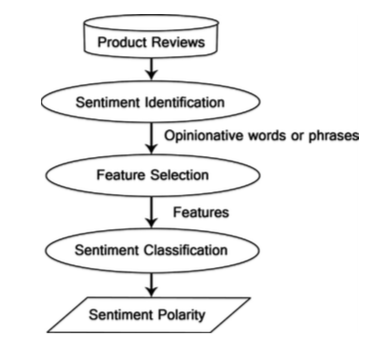
\includegraphics[width=0.4\textwidth]{./chapters/chapter1/images/sa_process}
\caption{Sentiment analysis process on product reviews\cite{survey}}
\label{fig:sa_process}
\end{figure}

There are three main classification levels in SA: 
\begin{itemize}
\item Document-level
\item Sentence-level
\item Aspect-level
\end{itemize}
Their difference is the granularity at which they operate. Indeed, while document-level SA aims to classify a document as expressing a positive or negative opinion or sentiment by considering the whole document as the basic information unit, sentence-level SA aims at classifying the sentiments/opinions expressed in each sentence.
In both cases the first step is to identify whether the sentence/document is subjective or objective and if it is subjective determine whether the sentence expresses positive or negative opinions. \par

In certain applications, classifying text at the document level or at the sentence level may not provide the necessary details needed for detecting opinions on all aspects of the entity. Aspect-level SA, instead, aims at classifying the sentiment with respect to the specific aspects of entities. The first step is to identify the entities and their aspects. Then, all the different opinions on the same entity must be considered. Indeed, the opinion holders may also give different opinions for different aspects of the same entity, e.g. ``This chair is ugly but it is comfortable''.

Sentiment Analysis task is considered as a sentiment classification (SC) problem. The first step in the SC problem is to extract and select text features. Some of the most commonly used features are:
\begin{itemize}
\item \textbf{Terms presence and frequency}: These features are individual words or word n-grams and their frequency counts;
\item \textbf{Parts of speech (POS)}: finding adjectives, pronouns, etc. as they are important indicators of opinions;
\item \textbf{Opinion words and phrases}: these are words commonly used to express opinions including \textit{good or bad, like or hate}. On the other hand, some phrases express opinions without using opinion words, e.g. \textit{cost me and arm and a leg};
\item \textbf{Negations}: the appearance of negative words may change the opinion orientation like \textit{not good} is equivalent to \textit{bad}. 
\end{itemize}

Sentiment Classification techniques can be roughly divided into machine learning approach, lexicon based approach and hybrid approach\cite{survey}. \par

The \textit{Machine Learning Approach (ML)} applies the famous ML algorithms and uses linguistic features. 

The \textit{Lexicon-based Approach} relies on a sentiment lexicon, a collection of known and precomiled sentiment terms. It is divided into dictionary-based approach and corpus-based approach which use statistical or semantic methods to find sentiment polarity.

The \textit{Hybrid Approach} combines both approaches. 

The various approaches and the most popular algorithms of SC are illustrated in Fig \ref{fig:sentiment_classification}. 

\begin{figure}[H]
\centering
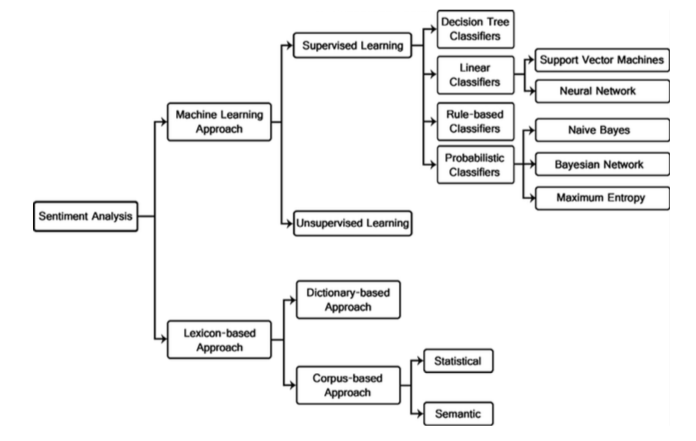
\includegraphics[width=0.8\textwidth]{./chapters/chapter1/images/sentiment_classification}
\caption{Sentiment classification techniques\cite{survey}}
\label{fig:sentiment_classification}
\end{figure}

The text classification methods using ML approach can be roughly divided into supervised and unsupervised learning methods. The supervised methods make use of a large number of labeled training documents. The unsupervised methods are used when it is difficult to find these labeled training training documents. \par
The lexicon-based approach depends on finding the opinion lexicon which is used to analyze the text. There are two methods in this approach:

\begin{itemize}
\item Dictionary-based
\item Corpus-based
\end{itemize}

In the Dictionary-based approach a small set of opinion words is collected manually with known orientations. Then, this set is grown by searching their synonyms and antonyms. The newly found words are added to the seed list then the next iteration starts. The iterative process stops when no new words are found. The dictionary based approach has a major disadvantage which is the inability to find opinion words with domain and context specific orientation. 

The limitation of the dictionary-based approach is addressed by the corpus-based approach, which depends on syntactic patterns or patterns that occur together along with a seed list of opinion words to find other opinion words in a large corpus. One of these methods is called \textit{sentiment consistency}: it starts with a list of seed opinion adjectives, and used them along with a set of linguistic constraints to identify additional adjective opinion words and their orientations. The constraints being for example \textit{AND, OR, BUT, EITHER-OR,...}; the conjunction \textit{AND} for example says that conjoined adjectives usually have the same orientation. \par

\section{Emotion Detection}

Emotion detection (ED) is the process of identifying human emotions. It is a recent field of research that is closely related to Sentiment Analysis. Indeed, Sentiment Analysis aims to detect positive, neutral or negative feelings from text, whereas Emotion Analysis aims to detect and recognize feelings in natural language texts. Therefore we can look at ED as a finer grained task with respect to SA.\par
Emotion is expressed as joy, sadness, anger, surprise, hate, fear and so on. Since there is not any standard emotion word hierarchy, the focus is on the related research about emotion in cognitive psychology domain. In 2001, W. Gerrod Parrot, wrote a book named ``Emotions In Social Psychology''\cite{Parrott2016}, in which he explained the emotion system and formally classified the human emotions through an emotion hierarchy in six classes at primary level which are \textit{Love, Joy, Anger, Sadness, Fear and Surprise} \cite{edfromtext}.\par

Emotion detection may have useful applications, such as \cite{microsoft}: 
\begin{itemize}
\item Measure citizens happiness;
\item Pervasive computing: this may include suggesting help when anxiety is detected through speech, or to check the tone of an email; 
\item Improving perception of a customer to increase brand reputation and sales. 
\end{itemize}

Some of the biggest challenges in determining emotion are:
\begin{itemize}
\item \textit{Context-dependence of emotions}: people use different regulation strategies in different social contexts. A phrase can have element of \textit{anger} without using the word ``anger'' or any of its synonyms, e.g. \textit{``Shut up!''}
\item \textit{Word-sense disambiguation}: identifying which sense a word (i.e. its meaning) is used in a sentence, when the word has multiple meanings; 
\item \textit{Co-reference resolution}: pronouns and other referring expressions must be connected to the right individuals;
\item Lack of labelled emotion databases. 
\end{itemize}

The main methods used for text based emotion detection are: 
\begin{itemize}
\item \textit{Keyword Spotting}
\item \textit{Lexical Affinity}
\item \textit{Learning-based}
\item \textit{Hybrid}
\end{itemize}

\paragraph{Keyword Spotting}
The keyword pattern matching problem can be described as the problem of finding occurrences of keywords from a given set as substrings in a given string. These words are classified into categories such as disgusted, sad, happy, angry, fearful, surprised, etc. The process of Keyword spotting method is  shown in Fig \ref{fig:keyword_spotting}. 

\begin{figure}[H]
\centering
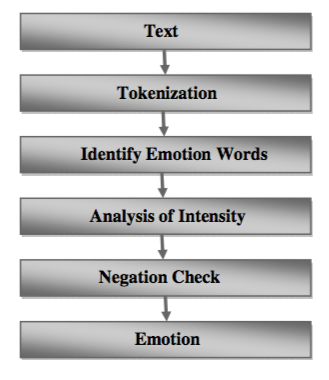
\includegraphics[width=0.4\textwidth]{./chapters/chapter1/images/keyword_spotting}
\caption{Keyword spotting technique}
\label{fig:keyword_spotting}
\end{figure}

The first step is converting data into tokens, i.e. a sentence into words, then from these tokens emotion words are detected. The second step is analyzing the intensity of emotion words. Sentence, then, is checked whether negation is involved in it or not then finally an emotion class will be assigned.

\paragraph{Lexical Affinity method} 
The Lexical Affinity approach is an extension of keyword spotting technique: apart from picking up emotional keywords it assigns \textit{probabilistic affinity} for a particular emotion to arbitrary words. This technique has the main disadvantage of missing out emotion content that resides deeper than the word level.\\
For example the word 'accident', having been assigned a high probability of indicating a negative emotion, would not contribute correctly to the emotional assessment of phrases like \textit{``I avoided an accident''} or \textit{``I met my girlfriend by accident''}. 

\paragraph{Learning-based methods}
Learning-based methods change the focus from ``determining emotions'' to ``classify the input texts into different emotions''. Indeed, learning-based methods try to detect emotions based on a previously trained classifier, which apply various theories of machine learning such as Support Vector Machines (SVMs).

\paragraph{Hybrid Methods}
Since keyword-based methods and na\"{i}ve learning-based methods could not acquire satisfactory results, some systems use hybrid approach by combining both keyword spotting technique and learning based method, which help to improve accuracy. \\
\\

However all these methods have some major limitations:
\begin{itemize}
\item \textit{Ambiguity in Keyword Definitions}: words can have multiple and vague meanings that can change according to different usages and contexts. Moreover emotion labels could have different emotions in some extreme cases such as ironic or cynical sentences; 
\item \textit{Lack of Linguistic Information}: these methods totally ignore syntax structures and semantics that also have influences on expressed emotions. For example the sentences \textit{``He laughed at me''} or \textit{``I laughed at him''} express two totally different meanings;
\item \textit{Incapability of Recognizing Sentences without Keywords}: sentences without any keyword would imply that they do not contain any emotion at all, which is obviously wrong. 
\end{itemize}

Deciding a way to label emotions is another challenging aspect of ED. There are mainly two possible ways to label data \cite{microsoft}:
\begin{enumerate}
\item The label is one between the set of emotions, e.g. \textit{anger, disgust, sad, happy, surpise, fear, neutral};
\item \textit{Slider approach}: the label is composed of percentages for each emotion, as described in Fig \ref{fig:emotion_labeling_sliders}.
\end{enumerate}

\begin{figure}[H]
\centering
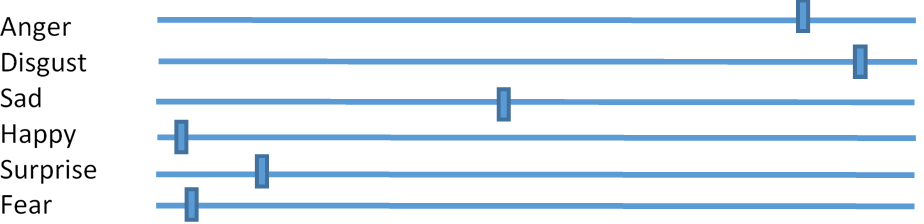
\includegraphics[width=0.8\textwidth]{./chapters/chapter1/images/emotion_labeling_sliders}
\caption{Slider approach\cite{microsoft}}
\label{fig:emotion_labeling_sliders}
\end{figure}

The sliders approach certainly offers more information but it comes with additional computational complications. However, the probabilistic assignment produced in the sliders approach can be turned into distinct labels of single emotions, just like those produced by first labeling approach, but of course, we can not move from the first approach to the second one. 


\chapter{Problem Pre-processing}
\section{The problem}
The goal of the semester project is to unravel the emotion pattern underlying the sequences of songs in a playlist using automatic approaches of Emotion Detection on the lyrics.\par
The problem can be divided into two main parts:
\begin{enumerate}
\item Classify emotions for each song based on the lyrics
\item Analyze emotion patterns in the playlists
\end{enumerate}

\section{Related work}
Emotion detection domain has already attracted many researchers from computer science, psychology, cognitive science and so on. \par
Before building our own emotion detection system we start analyzing some already existent classifier. \par
\paragraph{IBM Watson Natural Language Understanding}\cite{ibm_watson}
Watson is a question answering computer system capable of answering questions posed in natural language, developed by IBM.\par
Natural Language Understanding is a collection of APIs that allows to:
\begin{itemize}
\item Recognize the overall sentiment, in a scale from negative to positive [-1, 1];
\item Detect the emotion percentage between: joy, anger, disgust, sadness, fear;
\item Determine keywords ranked by relevance;
\item Extract entities: people, companies, organizations, cities and other information;
\item Classify content into hierarchical categories;
\item Identify general concepts that may not be directly referenced in the text; 
\end{itemize}
Results obtained analyzing Oasis - Wonderwall are illustrated in Fig.


\paragraph{IBM Watson Tone Analyzer}\cite{ibm_watson_tone}
It uses linguistic analysis to detect joy, fear, sadness, anger, analytical, confident, and tentative tones found in text. It allows to select different sources: tweets, online reviews, email messages, or other text. It uses both:
\begin{itemize}
\item the document level: to get a sense of the overall tone;
\item the sentence level: to identify specific areas where tones are the strongest.
\end{itemize}

\paragraph{QEmotion}\cite{qemotion}
Qemotion detects the main emotion of the speech and define the corresponding emotion in terms of temperature. 
\begin{itemize}
\item From $31^{\circ}$ to $40^{\circ}$ $\to$ Happiness
\item From $21^{\circ}$ to $30^{\circ}$ $\to$ Surprise
\item From $11^{\circ}$ to $20^{\circ}$ $\to $ Calm
\item From $6^{\circ}$ to $10^{\circ}$ $\to $ Fear
\item From $-5^{\circ}$ to $5^{\circ}$ $\to $ Sadness
\item From $-14^{\circ}$ to $-6^{\circ}$ $\to $ Anger
\item From $-20^{\circ}$ to $-15^{\circ}$ $\to $ Disgust
\end{itemize}


\section{NLP libraries}
In order to select the best Natural Language Processing library for our purpose we also analyzed pros and cons of the main Natural Language Processing libraries, i.e. NLTK, TextBlob, Standord's CoreNLP and SpaCy. 

\paragraph{NLTK: Natural Language Toolkit}
It is recommended only as an education and research tool. \\
Pros:
\begin{itemize}
\item its modularized structure makes it excellent for learning and exploring NLP concepts; 
\item over 50 corpora and lexicons, 9 stemmers, and a dozens of algorithms to choose from (this can also be considered as a con).
\end{itemize}
Cons: 
\begin{itemize}
\item Heavy library with a steep learning curve;
\item Slow and not production-ready. 
\end{itemize}

\paragraph{TextBlob}
Built on top on NLTK.\\
Pros: 
\begin{itemize}
\item More intuitive; 
\item Gentle learning curve. 
\end{itemize} 

\paragraph{Stanford's CoreNLP}
Java library with Python wrappers. \\
Pros:
\begin{itemize}
\item fast;
\item support for several major languages. 
\end{itemize}

\paragraph{SpaCy}
It is a new NLP library designed to be fast, streamlined and production-ready.\\
Pros:
\begin{itemize}
\item minimal number of options;
\item its philosophy is to only present the best algorithm for each purpose. 
\end{itemize}
Cons:
\begin{itemize}
\item it is new, so its support community is not as large as other libraries, but it is growing very fast.
\end{itemize}





\section{Word embedding techniques}
Word embeddings are a set of feature learning techniques mapping words or phrases from the vocabulary to vectors or real numbers. \par
These techniques map sparse word vectors into continuous space based on the surrounding context. For example if \textit{``salt''} and \textit{``seasoning''} appear within the same context, the model will indicate that \textit{``salt''} is conceptually closer to \textit{``seasoning''}, than another word, say \textit{``chair''}.\par
There are two main embedding libraries: Word2vec and FastText. While Word2vec treats each word in corpus like an atomic entity generating a vector for each word, FastText treats each word as composed of character ngrams, so the vector for a word is made of the sum of this character n grams. \par
For example,  the word vector \textit{``apple''} is a sum of the vectors of the n-grams ``ap'', ``app'', ``appl'', ``apple'', ``ppl', ``pple'', ``ple'', ``le'' assuming 3 and 6 as minimum and maximum ngrams size.\\
The difference between Word2vec and FastText manifests as follows:
\begin{enumerate}
\item \textit{Rare words}: even if words are rare, their character n-grams are still shared with other words - hence the embeddings with FastText can still be good;
\item \textit{Out of vocabulary words}: FastText can construct the vector for a word from its character n-grams even if word does not appear in training corpus;
\item \textit{Hyperparameters choice}: FastText requires to  choose the minimum and maximum n-grams sizes, and this directly impacts the computation time and the memory requirements. 
\end{enumerate}




\section{Public datasets}
A big challenge in emotion detection is the lack of a labelled emotion database to enable active innovation. Currently, few publicly accessible databases are available.\\\textit{MoodyLyrics}\cite{moodylyrics} contains around 2500 songs manually annotated through Amazon Mechanical Turk with 4 different emotion, i.e., happy, sad, angry and relaxed.\\
\textit{EmoInt}\cite{emoint} contains manually annotated tweets classified according to the intensities of anger, fear, joy and sadness. \textit{EmoBank}\cite{emobank} instead contains 10.000 sentences, each of which has been annotated according to both the emotion expressed by the writer and the emotion perceived by the reader. 
















\chapter{Emotion Classification Approaches}

In this chapter we will go through the experiments we made for this
project. Specifically, we will show how we tried to build some first models, solely 
based on the MoodyLyrics dataset, with no particular preprocessing nor feature
engineering techniques, just by using the tools we already mentioned. Then we will
move to more complex feature engineering techniques and classifiers.

Along with that, we will also provide a formal validation of one of the tools we used, in
order to make sure that what we have at our disposal is good for our task.

%%%%%%%%%%%%%%%%%%%%%%%%%%%%%%%%%%%%%%%%%%%%%%%%%
%%%%%%%%%%%%%%%%%%%%%%%%%%%%%%%%%%%%%%%%%%%%%%%%%
%%%%%%%%%%%%%%%%%%%%%%%%%%%%%%%%%%%%%%%%%%%%%%%%%
%%%%%%%%%%%%%%%%%%%%%%%%%%%%%%%%%%%%%%%%%%%%%%%%%
%%%%%%%%%%%%%%%%%%%%%%%%%%%%%%%%%%%%%%%%%%%%%%%%%
\section{Public datasets}
A big challenge in emotion detection is the lack of a labelled emotion database to enable active innovation. Currently, few publicly accessible databases are available.\\\textit{MoodyLyrics}\cite{moodylyrics} contains around 2500 songs manually annotated through Amazon Mechanical Turk with 4 different emotion labels, i.e., happy, sad, angry and relaxed.\\
\textit{EmoInt}\cite{emoint} contains manually annotated tweets classified according to the intensities of anger, fear, joy and sadness. \textit{EmoBank}\cite{emobank} instead contains 10.000 sentences, each of which has been annotated according to both the emotion expressed by the writer and the emotion perceived by the reader.

Certainly, the most appropriate dataset for our problem among those we found is MoodyLyrics.

\subsection{MoodyLyrics}

As already mentioned, MoodyLyrics is a manually annotated dataset of 2595 songs labeled according to 4
different emotion labels: happy, sad, angry and relaxed.

MoodyLyrics creators used content words of lyrics and their valence and arousal norms to assign songs with those labels.
In particular, they used Russell's Valence-Arousal model with the 4 mood categories described for the annotation process\cite{russell1980circumplex}. Valence, which describes the pleasant-unpleasant degree, and Arousal, which describes aroused-sleepy degree, values of songs are computed adding the corresponding values of each word of lyrics that is found in a lexicon which was build by combining ANEW (Affect Norm of English Words), WordNet and WordNet-Affect. 

In the context of MoodyLyrics, Valence represents the positive or negative intensity of an emotion whereas Arousal indicates how strongly or rhythmically the emotion is felt\cite{moodylyrics}.

Based on this assumptions, MoodyLyrics creators classified lyrics according to the planar model shown in figure \ref{fig:ml-classification-schema}, which relates arousal and valence.

\begin{figure}
  \centering
  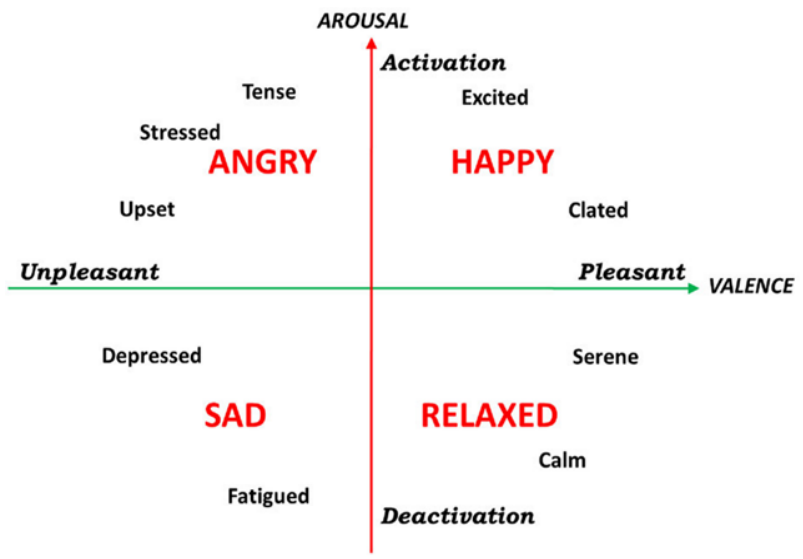
\includegraphics[width=0.9\textwidth]{./chapters/chapter4/images/moodylyrics-classification-schema}
  \caption{Valence and Arousal planar model used by MoodyLyrics creators to annotate lyrics\cite{moodylyrics}}
  \label{fig:ml-classification-schema}
\end{figure}

\subsubsection{MoodyLyrics duplicates bug}

During the analysis of MoodyLyrics described in the previous section we detected the presence of duplicated songs inside the dataset. Moreover, sometimes different emotions were associated with the duplicated songs. Thus, to continue our analysis we eliminated duplicated rows and we chose as emotion label the most frequent emotion between all the duplicates.\par

This bug in the dataset was reported to MoodyLyrics creators. As a response to our bug report email, MoodyLyrics creators suggested to use MoodyLyrics4Q\cite{moodylyrics4q}, that, according to them is a more accuratelly labeled version of MoodyLyrics.\par

This advice opened us three possibilities: continue using MoodyLyrics, start using MoodyLyrics4Q or create a new dataset as the concatenation of the previous two. We decided to start using all these three models, in order to understand which one, at the end, will give us a better playlists classification. The complete MoodyLyrics emotion classification analysis can be found at \url{https://github.com/sgiammy/emotion-patterns-in-music-playlists/blob/master/Notebook/1_ED_in_songs_lyrics.ipynb} while the MoodyLyrics4Q and the emotion detection analysis in the merged datasets can be found at \url{https://github.com/sgiammy/emotion-patterns-in-music-playlists/blob/master/Notebook/2_Advanced_Feature_Engineering.ipynb}.


\subsection{MoodyLyrics4Q}
MoodyLyrics4Q contains 2000 songs and has the same annotation schema as MoodyLyrics. Figure \ref{fig:stats}
shows the emotions distribution comparison between the two MoodyLyrics versions.

\begin{figure}[H]
\centering
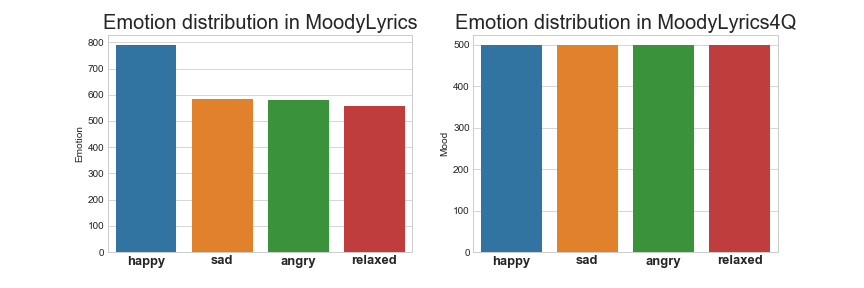
\includegraphics[width=1.1\textwidth]{./chapters/chapter4/images/Stats.png}
\caption{Emotions distribution comparison between MoodyLyrics and MoodyLyrics4Q}
\label{fig:stats}
\end{figure}

MoodyLyrics4Q classes are much more balanced, however MoodyLyrics4Q contains less songs with respect to MoodyLyrics. \par
We studied the qualitative difference between the two version comparing the classification given to the songs contained in both datasets to establish what version, according to us, is more correct. The intersection between the two versions contains 47 songs, and 21 over 47 have been classified differently. We noticed that in 15 over this 21 songs the two datasets confuses \textit{happy} with \textit{relaxed} and \textit{angry} with \textit{sad}. Indeed, only 6 of 21 songs are classified totally differently if we assume that we can merge happy and relaxed and angry and sad emotion. However, reading the lyrics of each of this 6 songs, we could not establish which version is the best one.

%%%%%%%%%%%%%%%%%%%%%%%%%%%%%%%%%%%%%%%%%%%%%%%%%
%%%%%%%%%%%%%%%%%%%%%%%%%%%%%%%%%%%%%%%%%%%%%%%%%
%%%%%%%%%%%%%%%%%%%%%%%%%%%%%%%%%%%%%%%%%%%%%%%%%
%%%%%%%%%%%%%%%%%%%%%%%%%%%%%%%%%%%%%%%%%%%%%%%%%
%%%%%%%%%%%%%%%%%%%%%%%%%%%%%%%%%%%%%%%%%%%%%%%%%
\section{POS Tagger Validity Check} 

Before digging into more complex types of analysis, we took the time to check if
the tools we were using could be really good for our purpose. 

Specifically, we had some doubts on the Part-Of-Speech (POS) tagger. Indeed, those kind of systems are generarly 
trained on texts coming from sources whose type of language is very different from those
we would expect to find in lyrics. In fact, the SpaCy's POS tagger implemented in the language
model we are using is trained on OntoNotes 5\cite{ontonotes5} and on Common Crawl\cite{common-crawl},
which are both made of pieces of text taken from news, conversational telephone speech, weblogs, 
usenet newsgroups, broadcast and talk shows. Obviously, this type of natural language texts are 
much different from a lyric and we just wanted to make sure that we were using an appropriate tool.

Before going into the details of what we did, we must state that SpaCy's POS tagger provides two tags per words, which
will both be considered in our analysis. Those two types of tag are:

\begin{itemize}
\item \textbf{POS}: coarse-grained part-of-speech e.g. VERB
\item \textbf{TAG}: fine-grained part-of-speech e.g. PAST\_TENSE
\end{itemize}

In order to obtain reliable insights of the functionalities of our POS tagger we considered three songs:
one with a common language and very few slang words, one filled with slangs and another one with some
vulgar words.

The first song we considered was ``Polly'' from Nirvana.

As a first approach we tried to tag the words considering one line of the lyric at the time. Here is an example of
what we obtained:

\begin{lstlisting}
Polly wants a cracker
PROPN VERB DET NOUN 

Polly = PROPN NNP -> noun, proper singular
wants = VERB VBZ -> verb, 3rd person singular present
a = DET DT -> determiner
cracker = NOUN NN -> noun, singular or mass
\end{lstlisting}

As a first attempt, our POS tagger completelly succedeed in recognizing the phrase in the 
exact way we were expecting. In fact, the absence of weird words, e.g. slangs, made the
task much easier.

Because of the almost complete absence of punctuation marks in our lyrics, we expected
the POS tagger to fail while analyzing an entire song as whole. Instead, we were quite
surprised to see that SpaCy's POS tagger does one desirable thing for our goal:
it treats each line as a standalone sentence, even though they are not specifically separed by
a stopping mark. Therefore, the same positive behaviour we observed on the first line
was totally replicated on the other lines, giving us the exact tagging we were
expecting by visually inspecting our song's lyrics.

We omitted the entire tagging process output for brevity reasons.

Our first experiment served to the purpose of arriving to a conclusion: SpaCy's POS tagger
is a good tool for lyrics. However it did not solve our doubts about its ability of recognizing
"weirder" words such as slang words or abbreviations. For this reason, we moved on 
analysing the lyrics of ``Kiss You Back'', from Underground Kiss.

The first interesting thing we noticed was that the POS tagger properly recognized abbreviations such as "'ll".
Moreover, another important feature we noticed was clearly visible while tagging this line: ``Yeah, we chocolate cross-over''.
Indeed, here the word "chocolate" is used as a verb (even though chocolate is clearly not defined as a verb in 
the dictionary) and the POS tagger was able to recognize this exception. 
This is quite important because, in songs, those situations happen very often.

Other additional things we noticed while analyzing this song came our of the tagging output of the following line:

\begin{lstlisting}
Jus't havin' fun with it, man, know what I'm sayin'?
NOUN VERB NOUN ADP PRON PUNCT INTJ PUNCT VERB NOUN PRON VERB VERB PUNCT PUNCT 

Jus't = NOUN NNS -> noun, plural
havin' = VERB VBG -> verb, gerund or present participle
fun = NOUN NN -> noun, singular or mass
with = ADP IN -> conjunction, subordinating or preposition
it = PRON PRP -> pronoun, personal
, = PUNCT , -> punctuation mark, comma
man = INTJ UH -> interjection
, = PUNCT , -> punctuation mark, comma
know = VERB VB -> verb, base form
what = NOUN WP -> wh-pronoun, personal
I = PRON PRP -> pronoun, personal
'm = VERB VBP -> verb, non-3rd person singular present
sayin = VERB VBG -> verb, gerund or present participle
' = PUNCT '' -> closing quotation mark
? = PUNCT . -> punctuation mark, sentence closer
\end{lstlisting}

One very interesting result we can notice comes from the following two lines:
\begin{lstlisting}
havin' = VERB VBG -> verb, gerund or present participle and
ayin = VERB VBG -> verb, gerund or present participle
\end{lstlisting}

In fact it looks like our POS tagger is able to recognize verbs in their correct tense
even if they are abbreviated in an unconventional way.

One thing which really impressed us, was the word "man" being recognized to be an interjection from time to time. 
"An interjection is a part of speech that shows the emotion or feeling of the author. These words or phrases can 
stand alone or be placed before or after a sentence. Many times an interjection is followed 
by a punctuation mark, often an exclamation point"\footnote{\url{http://examples.yourdictionary.com/examples-of-interjections.html}}. 
This description perfectly fits with the usage of the word "man" in their contextes when it was recognized to be an interjection. 

Those kind of things are not trivial to detect and this ability of our POS tagger convinced us even more
of its impressive skills.

The last thing we were left to analyze at this point was a vulgar song. For this purpose we considered 
"The Ballad Of Chasey Lain", from Bloodhound Gang. 

In this case we have no special remarks to report. We can just say that everything was tagged and
recognized in the exact way we expected.

We did not report entire lyrics nor the full POS tagger output in the interest of brevity. However, those
analysis are available on the public GitHub repository for this project\footnote{\url{https://github.com/sgiammy/emotion-patterns-in-music-playlists/blob/master/Notebook/3\_POS\_tagger\_verification.ipynb}}.

%%%%%%%%%%%%%%%%%%%%%%%%%%%%%%%%%%%%%%%%%%%%%%%%%
%%%%%%%%%%%%%%%%%%%%%%%%%%%%%%%%%%%%%%%%%%%%%%%%%
%%%%%%%%%%%%%%%%%%%%%%%%%%%%%%%%%%%%%%%%%%%%%%%%%
%%%%%%%%%%%%%%%%%%%%%%%%%%%%%%%%%%%%%%%%%%%%%%%%%
%%%%%%%%%%%%%%%%%%%%%%%%%%%%%%%%%%%%%%%%%%%%%%%%%
\section{Initial Classification}

The first approaches to classify emotions we tried, were entirely based on converting
MoodyLyrics entries into features. Specifically, since MoodyLyrics simply provides the
artist and the title of its songs, we firstly downloaded the lyrics and then we built
word embedding vectors for them by using SpaCy's built-in methods, based on Word2Vec.
Those vectors we worked on are made of 300 dimensions.

No particular preprocessing was applied on lyrics before generating the word embedding
vectors apart from stopword removals, because we did not believe that they could bring
any useful additional information.

\begin{figure}
  \centering
  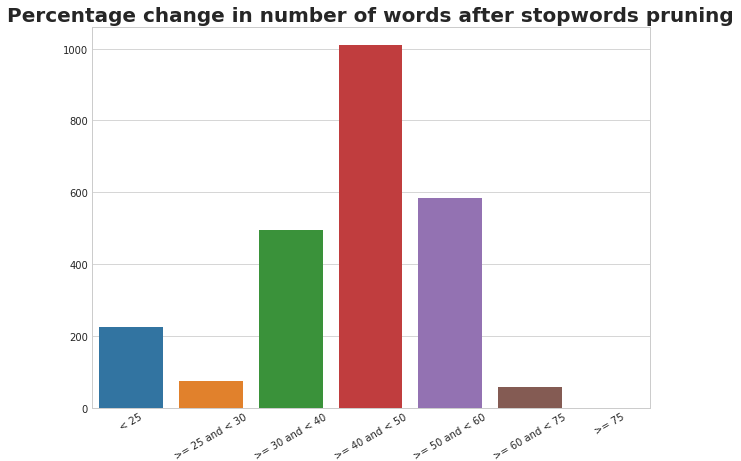
\includegraphics[width=0.9\textwidth]{./chapters/chapter4/images/percentage-change.png}
  \caption{Number of songs and percentage of word in which they changed after stop word removal}
  \label{fig:ml-percentage-change}
\end{figure}

At first we were scared of the fact that most of the words in some lyrics may have been
stop words, ending up in reducing lyrics text by too many words. Anyway, as we can see 
from figure \ref{fig:ml-percentage-change}, less than 650 songs reduced their size by 
more than 50\% while the majority of them has very small percentage decrease. Therefore
we concluded that it could be worth trying to classify our lyrics by applying this mentioned
preprocessing technique.

\begin{figure}
  \centering
  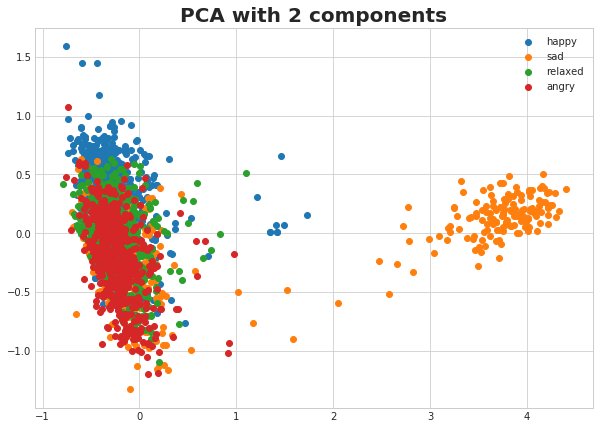
\includegraphics[width=0.9\textwidth]{./chapters/chapter4/images/ml-pca.png}
  \caption{Principal Component Analys on MoodyLyrics data with 2 dimensions as output}
  \label{fig:ml-pca}
\end{figure}

MoodyLyrics songs were annotated according to the arousal and valence dimension of their lyric,
as explained above. Therefore we tought that, if we could be able to project the resulting
word embedding vector of each lyric in a bi-dimensional space, we could have been able to 
clearly see how they are separated.

In order to visualize the mentioned idea, we applied Principal Component Analysis (PCA) on
MoodyLyrics songs and plotted the resulting points in 2-dimensional space, as can be seen in 
figure \ref{fig:ml-pca}. However the resulting figure is not exactly what we were expecting.

Indeed, because of the explained MoodyLyrics annotation schema, we were expecting to see 4
clearly separated group of points. Instead, what we can see is that sad songs are clearly 
separated from the others while the songs belonging to the classes happy, angry and relaxed
are quite overlapped and can be easily confused between them.

Despite the fact that this result seemed weird, after listening to several songs and trying to
manually classify them according to their lyrics, we came to the conclusion that it is very
easy for a human to confuse happy, angry and relaxed song. Therefore, if we keep in mind that
MoodyLyrics was manually annotated, we can explain the anomaly in our plot as a consequence
of human error during the annotation process.

\begin{table}[]
\centering
\begin{tabular}{@{}lll@{}}
\toprule
\textbf{Classifier} & \textbf{Accuracy})   \\ \midrule
k-Nearest Neighbour & 82\%  \\
Support Vector Machine & 90\%  \\
Gradient Boost & 86\%  \\
Neural Network & 90.55\%  \\
\end{tabular}
\caption{Accuracy results for different classifiers on MoodyLyrics}
\label{table:ml-simple-results}
\end{table}

After this preliminary data analysis, we moved on producing models to actually classify our dataset.
The result of these process are visible in table \ref{table:ml-simple-results} where the reported
accuracy values were obtain after a 10-fold cross validation.

As we can see, the best results were certainly achieved by a Neural Network whose architecture was
as follows: one input layer with 60 neurons and sigmoid activation function, one hidden layer with
60 neurons and sigmoid activation function, one output layer with 4 neurons and softmax activation
function.

\begin{table}[]
\centering
\begin{tabular}{@{}lll@{}}
\toprule
\textbf{Classifier} & \textbf{Accuracy})   \\ \midrule
Support Vector Machine & 67\%  \\
Gradient Boost & 65\%  \\
Neural Network & 70\%  \\
\end{tabular}
\caption{Accuracy results for different classifiers on MoodyLyrics, using just the title's word embedding vector}
\label{table:ml-simple-results-title}
\end{table}

Anyway for certain songs we noticed that the expressed emotion could be easily guessed from its title. Therefore
we tried to build also songs titles word embedding vectors and classified them. The results of this operation are 
visible in table \ref{table:ml-simple-results-title}. Again, those results were obtained after a 10-fold cross-validation. 

\begin{table}[]
\centering
\begin{tabular}{@{}lll@{}}
\toprule
\textbf{Classifier} & \textbf{Accuracy})   \\ \midrule
Support Vector Machine & 91\%  \\
Neural Network & 54.14\%  \\
\end{tabular}
\caption{Accuracy results for different classifiers on MoodyLyrics, using both the lyric's and the title's word embedding vectors}
\label{table:ml-simple-results-both}
\end{table}

Moreover, performances obtained while building classifiers based on the songs title's word embedding vector only
did not improve with respect to the previous case. Therefore we decided
that, probably, we could have given a try at using both the title's and the lyric's word embedding information for each
song. What we did was to use both lyrics vectors and title vectors norm. The results of this process are shown in table \ref{table:ml-simple-results-both}.

For this case we did not try to learn the same number of classifiers as above because, based on the previous experiments, we noticed
that SVM and ANN should be the best algorithms for our problem. 

The accuracy values obtained in this experiment seem quite abnormal. Indeed,
while the SVM provides an accuracy score which is comparable to those obtained while using only the lyrics content, the ANN performances 
drastically decreased. However, we were expecting to obtain performances very similar to those we got while using just the lyrics content as, 
in  this case, we are basically adding one features (which is the norm of the title's word embedding vector).

In conclusion, the best and more stable performances were those obtained by learning our model solely on the lyrics word embedding vectors.
Those results are also quite encouraging and made us think that, with some more advanced feature engineering techniques,
we may be able to achieve even better results.

%%%%%%%%%%%%%%%%%%%%%%%%%%%%%%%%%%%%%%%%%%%%%%%%%
%%%%%%%%%%%%%%%%%%%%%%%%%%%%%%%%%%%%%%%%%%%%%%%%%
%%%%%%%%%%%%%%%%%%%%%%%%%%%%%%%%%%%%%%%%%%%%%%%%%
%%%%%%%%%%%%%%%%%%%%%%%%%%%%%%%%%%%%%%%%%%%%%%%%%
%%%%%%%%%%%%%%%%%%%%%%%%%%%%%%%%%%%%%%%%%%%%%%%%%
\section{Feature Engineering}
In order to improve our model performances, we focused our attention on feature engineering. Specifically we tried to extract stylometric, structural, orientation and vocabulary based features\cite{features}. Apart from this we also generated a word embedding vector of the words contained in each song's lyric by using SpaCy's\cite{spacy} pre-trained language model based on Word2Vec\cite{word2vec}.\par

Here is a comprehensive list of the features we extracted from our dataset, followed by a brief description:

\begin{description}
\item \textbf{Title\_vector}: word embedding vector of the song's title
\item \textbf{Lyric\_vector}: word embedding vector of the lyric content
\item \textbf{\%Rhymes}: defined as the percentage of the number of rhymes over the number of total lines. A rhyme is defined as a rhyme between two following lines
\item \textbf{Line\_count}: number of lines in the lyric
\item \textbf{Word\_count}: number of words in the lyric
\item \textbf{\%Past\_tense\_verbs}: defined as the the percentage of the number of past tense verbs over the total number of verbs
\item \textbf{\%Present\_tense\_verbs}: defined as the the percentage of the number of present tense verbs over the total number of verbs
\item \textbf{\%Future\_tense\_verbs}: defined as the the percentage of the number of future tense verbs over the total number of verbs, where future is just will + base form
\item \textbf{\%ADJ}: percentage of adjectives over the total number of words
\item \textbf{\%ADP}: percentage of adpositions (e.g. in, to, during) over the total number of words
\item \textbf{\%ADV}: percentage of adverbs (e.g. very, tomorrow, down, where, there) over the total number of words
\item \textbf{\%AUX}: percentage of auxiliaries (e.g. is, has (done), will (do), should (do)) over the total number of words
\item \textbf{\%INTJ}: percentage of interjections (e.g. psst, ouch, bravo, hello) over the total number of words
\item \textbf{\%NOUN}: percentage of nouns over the total number of words
\item \textbf{\%NUM}: percentage of numerals over the total number of words
\item \textbf{\%PRON}: percentage of pronouns (e.g. I, you, he, she, myself, themselves, somebody,...) over the total number of words
\item \textbf{\%PROPN}: percentage of proper nouns (e.g. Mary, John) over the total number of words
\item \textbf{\%PUNCT}: percentage of puntuctuation (e.g. ., (, ), ?) over the total number of words
\item \textbf{\%VERB}: percentage of verbs over the total number of words
\item \textbf{Selfish\_degree}: percentage of 'I' pronouns over the total number of pronouns
\item \textbf{\%Echoism}: percentage of echoism over the total number of words, where an echoism is either a sequence of two subsequent repeated words or the repetition of a vowel in a word
\item \textbf{\%Duplicate\_Lines}: number of lines duplicated across the lyric text
\item \textbf{isTitleInLyric}: boolean, true if the title string is also a substring of the lyric
\item \textbf{Sentiment}: sentiment between -1 and 1
\item \textbf{Subjectivity\_degree}: degree of subjectivity of the text
\end{description}

Since the word embedding vectors we generated had length 300, at the end we were able to obtain 623 distinct numerical features for each of the songs in our dataset.

\subsection{Feature Selection}

Having to deal with 623 different features for discriminating songs among 4 classes is probably exaggerated and many features may be redundant or may not bring any useful information to our goal. Indeed, after running many experiments, we tried to keep our models as simple as possible by trying to select the fewer number of features possible.

In the end, we obtained the best results just by using the following features: \textit{Lyric\_vector}, \textit{\%Echoisms}, \textit{\%Duplicate\_Lines}, \textit{isTitleInLyrc}, \textit{\%Past\_tense\_verbs}, \textit{\%Present\_tense\_verbs}, \textit{\%Future\_tense\_verbs}, \textit{\%ADJ}, \textit{\%PUNCT}, \textit{Sentiment} and \textit{Subjectivity\_degree}. This process of feature selection left us with just 310 distinct features per song.

%%%%%%%%%%%%%%%%%%%%%%%%%%%%%%%%%%%%%%%%%%%%%%%%%
%%%%%%%%%%%%%%%%%%%%%%%%%%%%%%%%%%%%%%%%%%%%%%%%%
%%%%%%%%%%%%%%%%%%%%%%%%%%%%%%%%%%%%%%%%%%%%%%%%%
%%%%%%%%%%%%%%%%%%%%%%%%%%%%%%%%%%%%%%%%%%%%%%%%%
%%%%%%%%%%%%%%%%%%%%%%%%%%%%%%%%%%%%%%%%%%%%%%%%%
\section{Beyond the lyrics dataset: EmoInt}

One major limitation we had to face during our work on this project was the shortage in terms of labeled data.
Indeed, most of the already labeled datasets which can be found online have been created for type of texts
which were much different from lyrics i.e. news items, blog posts, Facebook posts, tweets, etc.

In order to overcome this limitation we tought that, if we found a dataset whose items language is close enough
to the common lyrics language, we would have had some performance improvements in our classifiers. This is the
reason why we tried to combine our dataset together with EmoInt\cite{emoint}.

EmoInt provides several tweets annotated according to an emotion (anger, fear, joy, sadness) and to the degree 
at which the emotion is expressed in text. As EmoInt provide intensity levels together with emotion labels, 
we decided to take into account only those tweets for which the intensity was greater that 0.50 (50\%). 

Our original dataset, MoodyLyrics, contains "happy", "sad", "angry" and "relaxed" as labels. 
Therefore, in order to perform a sort of interjection with EmoInt, we used only the tweets corresponding to the anger, 
joy and sadness emotions, discarding those belonging to the fear emotion as we would not have been able to map them into
our original work.

Moreover, it is important to mention that EmoInt was manually annotated using Best-Worst Scaling (BWS)\cite{bws}, 
an annotation scheme proved to obtain very reliable scores. Therefore, we choose EmoInt because it looked
like a realiable choice.

As a single preprocessing technique, we dropped hashtags and removed the tag characters 
(e.g. "Hey @MrTwitter how are you? \#cool" became "Hey MrTwitter how are you?") because 
we had to compare tweets with songs and songs do not have those kind of things. Also, 
this sort of preprocessing should maximize the chances that everything is properly recognized by our POS tagger.

After having preprocessed EmoInt, we combined it to our lyrics based dataset (MoodyLyrics) and tried some different
modeling approaches to see if we could obtain any performance improvements.

After having performed several different trials, we came to the conclusion that the best subset of features
to use for our new dataset (MoodyLyrics + EmoInt) was the following: \textit{Lyric\_Vector}, \textit{Word\_Count}, 
\textit{\%Echoisms}, \textit{Selfish\_degree}, \textit{\%Duplicate\_Lines}, \textit{isTitleInLyric}, 
\textit{\%Present\_tense\_verbs}, \textit{\%Past\_tense\_verbs}, \textit{\%Future\_tense\_verbs},
\textit{\%ADJ}, \textit{\%PUNCT}, \textit{Sentiment} and \textit{Subjectivity\_degree}.

\begin{table}[]
\centering
\label{table:emoint-results}
\begin{tabular}{@{}lll@{}}
\toprule
\textbf{Classifier} & \textbf{Accuracy})   \\ \midrule
k-Nearest Neighbour & 46\%  \\
Support Vector Machine & 48\%  \\
Gradient Boost & 46\%  \\
Neural Network & 82.38\%  \\
Multinomial Na\"{i}ve Bayes Classifier & 49\%  \\ \bottomrule
\end{tabular}
\caption{Accuracy results for different classifiers on MoodyLyrics and EmoInt combined}
\end{table}

Using the data obtained as explained, we built several classifiers with which we obtained the results
shown in table \ref{table:emoint-results}. We split our dataset
in a training and a test part and the shown results are those obtained while classifying the test set.

As it was when we used MoodyLyrics alone, the best results were obtained by using a Neural Network.
This network had a very simple architecture: one input layer with sigmoid activation function and 120 neurons,
one hidden layer with softmax activation function and 60 neurons and an output layer with 4 neurons and softmax
activation function.

Anyway, it is quite clear that this approach did not lead us to real improvements over our previous cases.
This experiment served to the purpose of understanding that EmoInt is probably too much different from what 
we have classify and it may not improve our predictive abilities at all. Therefore we believed that the best
choice was to keep using a lyrics based dataset as it is MoodyLyrics.

%%%%%%%%%%%%%%%%%%%%%%%%%%%%%%%%%%%%%%%%%%%%%%%%%
%%%%%%%%%%%%%%%%%%%%%%%%%%%%%%%%%%%%%%%%%%%%%%%%%
%%%%%%%%%%%%%%%%%%%%%%%%%%%%%%%%%%%%%%%%%%%%%%%%%
%%%%%%%%%%%%%%%%%%%%%%%%%%%%%%%%%%%%%%%%%%%%%%%%%
%%%%%%%%%%%%%%%%%%%%%%%%%%%%%%%%%%%%%%%%%%%%%%%%%
\section{Results}
In this section we present a summary of the result obtained while predicting one of the four emotion labels \textit{relaxed}, \textit{happy}, \textit{sad}, \textit{angry}, using an artificial neural network, a support vector machine, a logistic regression and xgboost. The accuracies have been computed with a 5-fold cross validation. The presented results were computed using both MoodyLyrics4Q and the union of MoodyLyrics and MoodyLyrics4Q. Of course, all of the feature engineering approaches described above were applied.

Here we omitted MoodyLyrics alone results because, after several experiments, we noticed that MoodyLyrics creators were right when saying that their first version of the dataset should be used as a ground truth dataset because it contains unappropriate labelings which could deteriorate performances in real world cases.

All the implementation details can be found at \url{https://github.com/sgiammy/emotion-patterns-in-music-playlists/blob/master/Notebook/2_Advanced_Feature_Engineering.ipynb}.

\begin{table}[H]
\begin{tabular}{ |p{3cm}||p{1.5cm}|p{1.5cm}|p{1.5cm}|p{1.5cm}|  }
 \hline
 \multicolumn{5}{|c|}{5-fold Cross Validation Accuracy} \\
 \hline
 Dataset & ANN & LR &SVM & xgboost\\
 \hline
MoodyLyrics4Q  & 51\%    &55\% &  59\% & 56\%\\
Both together &   67\%  & 68\%   &69\% &63.7\%\\
\hline
\end{tabular}
\caption{Emotion detection accuracies} \label{tab:comparison}
\end{table}

\begin{figure}[H]
  \centering
  \begin{subfigure}[b]{0.49\linewidth}
    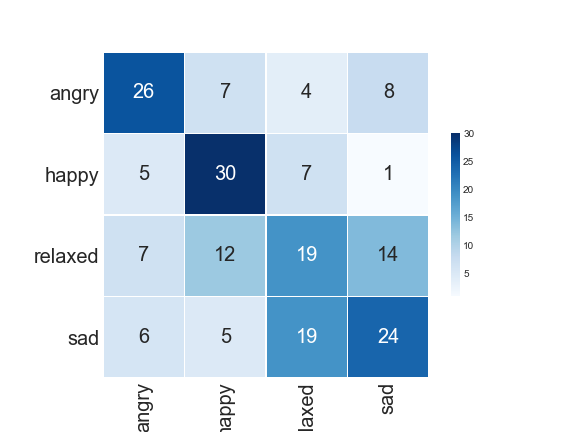
\includegraphics[width=\linewidth]{./chapters/chapter4/images/4Q/CM_ANN.png}
    \caption{ML4Q}
  \end{subfigure}
  \begin{subfigure}[b]{0.49\linewidth}
   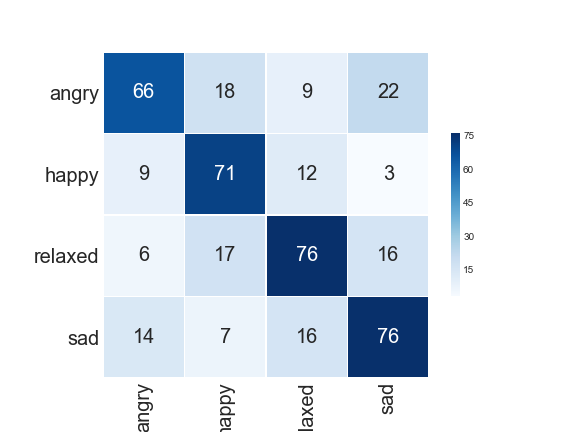
\includegraphics[width=\linewidth]{./chapters/chapter4/images/join/CM_ANN.png}
    \caption{ML + ML4Q}
  \end{subfigure}
  \caption{Artificial Neural Network - Confusion Matrix}
  \label{fig:ann}
\end{figure}

\begin{figure}[H]
  \centering
  \begin{subfigure}[b]{0.49\linewidth}
    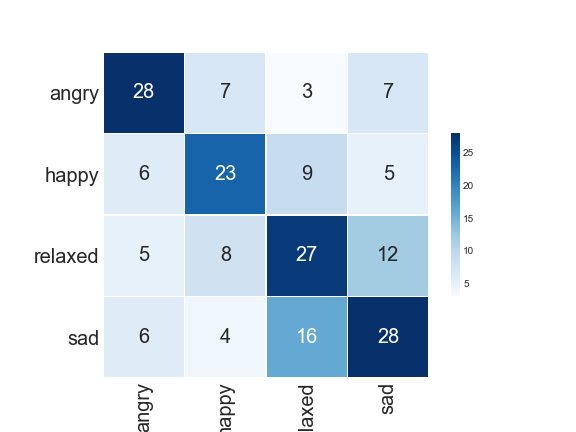
\includegraphics[width=\linewidth]{./chapters/chapter4/images/4Q/CM_LR.png}
    \caption{ML4Q}
  \end{subfigure}
  \begin{subfigure}[b]{0.49\linewidth}
   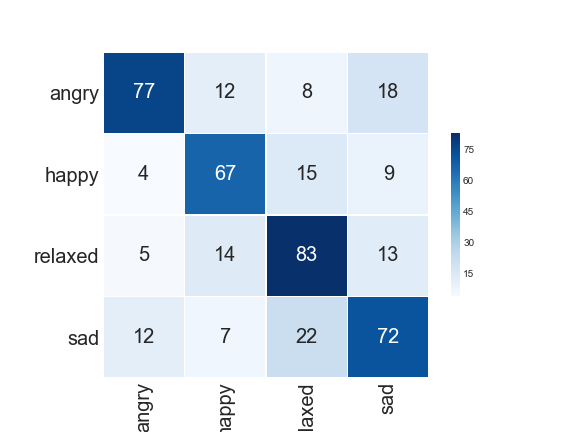
\includegraphics[width=\linewidth]{./chapters/chapter4/images/join/CM_LR.png}
    \caption{ML + ML4Q}
  \end{subfigure}
  \caption{Logistic Regression - Confusion Matrix}
  \label{fig:lr}
\end{figure}

\begin{figure}[H]
  \centering
  \begin{subfigure}[b]{0.49\linewidth}
    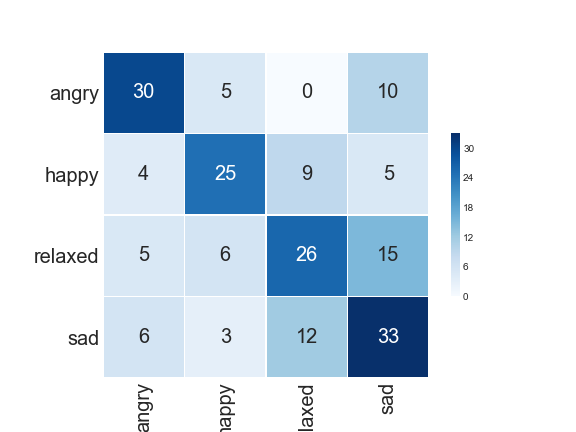
\includegraphics[width=\linewidth]{./chapters/chapter4/images/4Q/CM_SVM.png}
    \caption{ML4Q}
  \end{subfigure}
  \begin{subfigure}[b]{0.49\linewidth}
   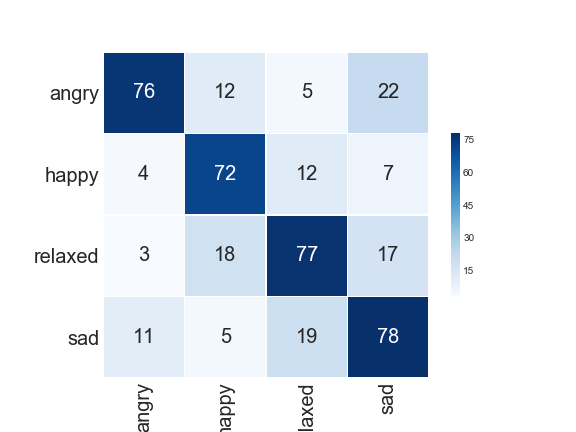
\includegraphics[width=\linewidth]{./chapters/chapter4/images/join/CM_SVM.png}
    \caption{ML + ML4Q}
  \end{subfigure}
  \caption{Support Vector Machine - Confusion Matrix}
  \label{fig:svm}
\end{figure}

\begin{figure}[H]
  \centering
  \begin{subfigure}[b]{0.49\linewidth}
    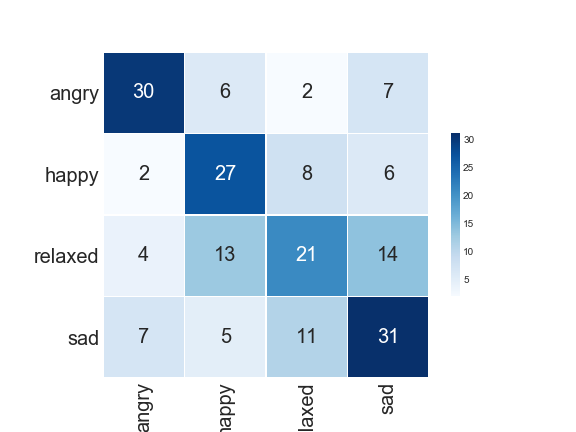
\includegraphics[width=\linewidth]{./chapters/chapter4/images/4Q/CM_XGB.png}
    \caption{ML4Q}
  \end{subfigure}
  \begin{subfigure}[b]{0.49\linewidth}
   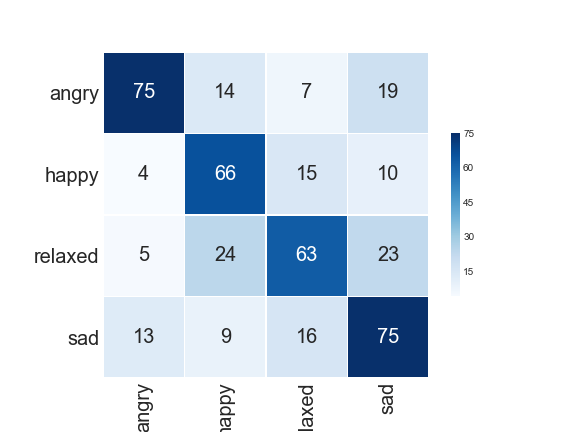
\includegraphics[width=\linewidth]{./chapters/chapter4/images/join/CM_XGB.png}
    \caption{ML + ML4Q}
  \end{subfigure}
  \caption{Xgboost - Confusion Matrix}
  \label{fig:xgb}
\end{figure}
\chapter{Playlists analysis}

Now we will move our focus from lyrics to playlists. Indeed, we will now demonstrate how we extended our work on single songs to whole playlists.

\section{Playlist classification}

Once we have a model for classifying song emotions, our next step it trying to classify playlists emotion which could be a really useful information for a Recommender System which want to perform playlist continuation.

For the emotion classification task we decided to use three artificial neural networks, with the same architecture, but trained with three different datasets: MoodyLyrics, MoodyLyrics4Q and the merged dataset. Figure \ref{fig:annacc} shows the different accuracies reached with each dataset.

\begin{figure}[H]
\centering
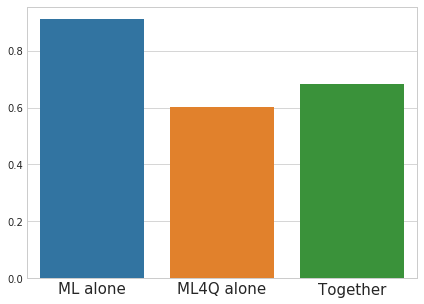
\includegraphics[width=0.7\textwidth]{./chapters/chapter5/images/ANN_accuracies.png}
\caption{5-fold ANN accuracies for each model}
\label{fig:annacc}
\end{figure}

Among the different classifiers we analyzed, we choose the neural network because we needed a probabilistic distribution as output of our classifier, and not just an hard assignment. This is the reason why we favoured neural networks over SVM and XGBoost algorithms, despite the fact that those gave better accuracy results.

Logistic regression seemed to give us slightly better results. However, we still decided to use the neural network over logistic regression as we believed that this last model is too simplistic, and may not perform well in real world situations.

The method we chose to classify a playlist is the following: given a \texttt{song emotion array} = [ sad\%, angry\%, happy\%, relaxed\% ] where the sum of the emotion percentage for each song is equal to one, the playlist emotion is the emotion with the maximum percentage column sum over the rows. We found this approach very flexible, indeed, normalizing by the number of songs inside a playlist we obtain a probability of the emotion for that playlist. This would add 4 additional features which could be used by a Recommendation System.

However our main issue has been the absence of a labeled dataset through which compute an accuracy score of our classification method. In order to overcome this problem a perfectly balanced silver standard dataset has been generated considering 40 playlist inside Spotify RecSys\cite{recsys} dataset with four really expressive titles: \textit{rage} for angry playlists, \textit{crying} for sad, \textit{party!} for happy and \textit{sleeping} for relaxed playlists. \par

The first step to classify the emotion for each song has been downloading the lyrics, but, unfortunately, we noticed that we could not download the entire number of song lyrics for every playlist. Figure \ref{fig:rsongs} shows, for each playlist, the number of songs for which we could download the lyrics, while figure \ref{fig:psongs} shows the percentage of available songs for each playlist. 

\begin{figure}[H]
\centering
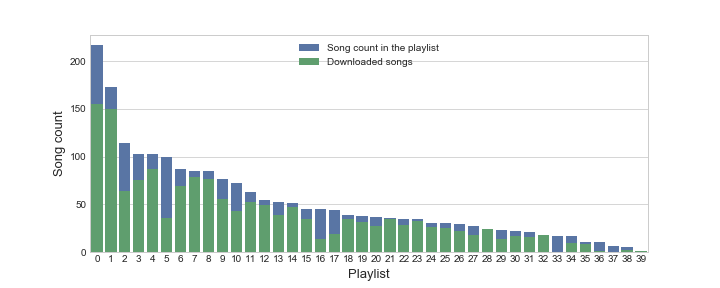
\includegraphics[width=1\textwidth]{./chapters/chapter5/images/silver_standard_available_songs.png}
\caption{Real number of available songs for playlist}
\label{fig:rsongs}
\end{figure}

\begin{figure}[H]
\centering
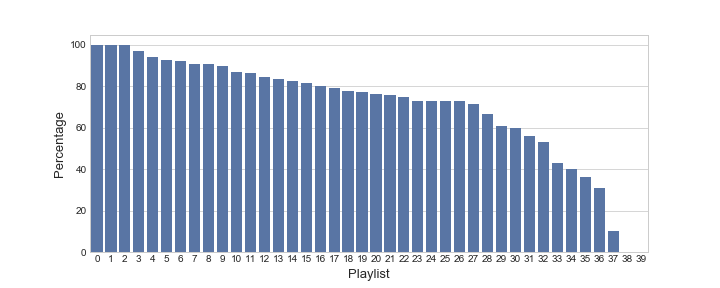
\includegraphics[width=1\textwidth]{./chapters/chapter5/images/silver_standard_percentage_available_songs.png}
\caption{Percentage of available songs for playlist}
\label{fig:psongs}
\end{figure}

Unfortunately two \textit{relaxed} playlist totally disappeared, unbalancing our silver standard.

We then featurized each song using the features described earlier in this report and classified them using the three artificial neural networks (one trained with MoodyLyrics, one with MoodyLyrics4Q and one with the merged datasets) we previously built.

\subsection{Robust Playlist Classification}

As we already said, playlist classification was done by averaging the emotion vectors which are given as output of the lyrics classification process. However, in order to make the classifications more robust, we tried to remove outliers from our predictions.

Basically, for each playlist, we built a matrix of dimension $N$x$4$, where $N$ is the number of songs in the playlist and $4$ is the number of target emotions (happy, sad, angry and relaxed). In this matrix, each row corresponds to the probabilistic assignment of emotions to each of song of the playlist. In order to remove outliers we considered a column (an emotion) at the time and we followed those steps:
\begin{enumerate}
\item compute the third (q3) and the first quartile (q1)
\item compute the interquartile range (IQR) defined as the difference between the third and the first quartile
\item define an upper bound value as $upper = q3 + (IQR * 1.5)$
\item define a lower bound value as $lower = q1 - (IQR * 1.5)$
\item eliminate from the column all those values outside the range $[lower, upper]$
\item average the remaining values to compute the label score for the emotion corresponding to the current column of the matrix
\end{enumerate}

After having repeated the above process for all the $4$ columns of our $N$x$4$ matrix, we obtain a vector of $4$ real values, respectively representing the playlist score for each of our target emotion.

\subsection{Playlist Classification with a subset of the songs}

In order to improve our computational speed we came up with the idea that probably a playlist's emotion is clearly expressed in just a subset of its songs, making it useless to compute emotion classification of each of its song. For this purpose, we tried to consider just a small sample of the total songs at the time, incrementally increasing our sample size.

We did this operation both using our simple, average based, classification scheme and the other, more robust, and outlier sensitive approach.

Figures \ref{fig:subset-absolute} and \ref{fig:subset-percentage} shows the accuracy results obtained while using the simple average classification approach, while figures \ref{fig:subset-absolute-robust} and \ref{fig:subset-percentage-robust} shows the results obtained while using the robust classification approach.

\begin{figure}[H]
\centering
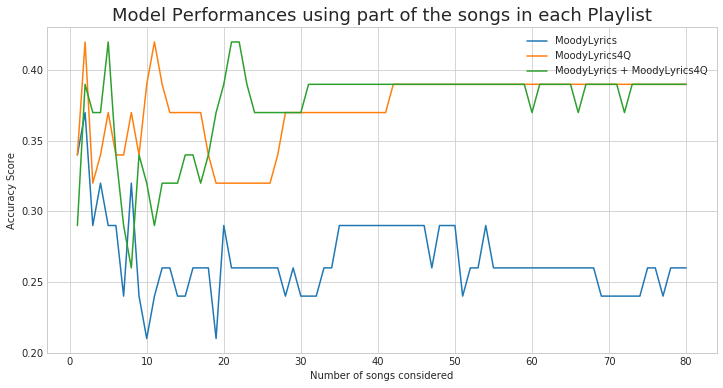
\includegraphics[width=0.9\textwidth]{./chapters/chapter5/images/subset-absolute}
\caption{Classification accuracy on playlists obtained while considering just a certain amount of songs}
\label{fig:subset-absolute}
\end{figure}

\begin{figure}[H]
\centering
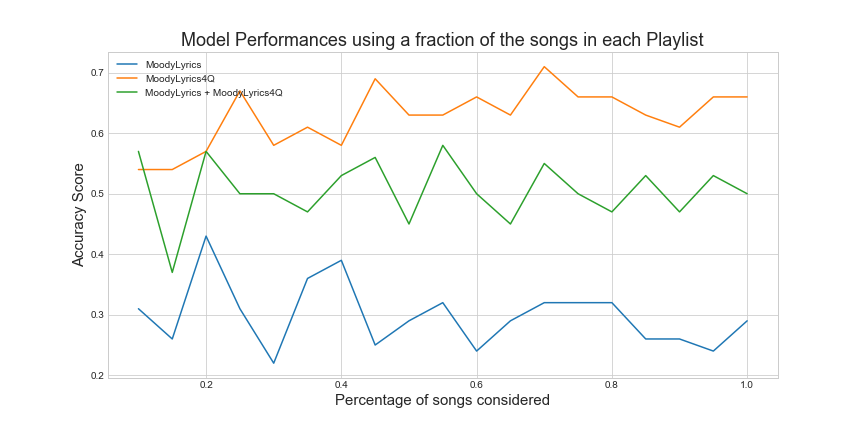
\includegraphics[width=0.9\textwidth]{./chapters/chapter5/images/subset-percentage}
\caption{Classification accuracy on playlists obtained while considering just a percentage sample of the total number of songs}
\label{fig:subset-percentage}
\end{figure}

\begin{figure}[H]
\centering
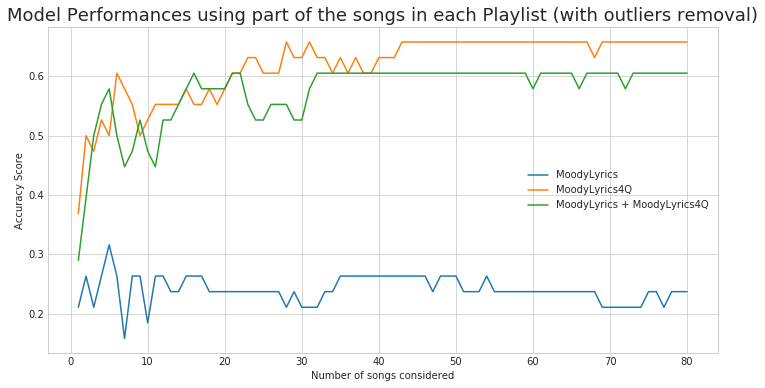
\includegraphics[width=0.9\textwidth]{./chapters/chapter5/images/subset-absolute-robust}
\caption{Classification accuracy on playlists obtained using robust classification while considering just a certain amount of songs}
\label{fig:subset-absolute-robust}
\end{figure}

\begin{figure}[H]
\centering
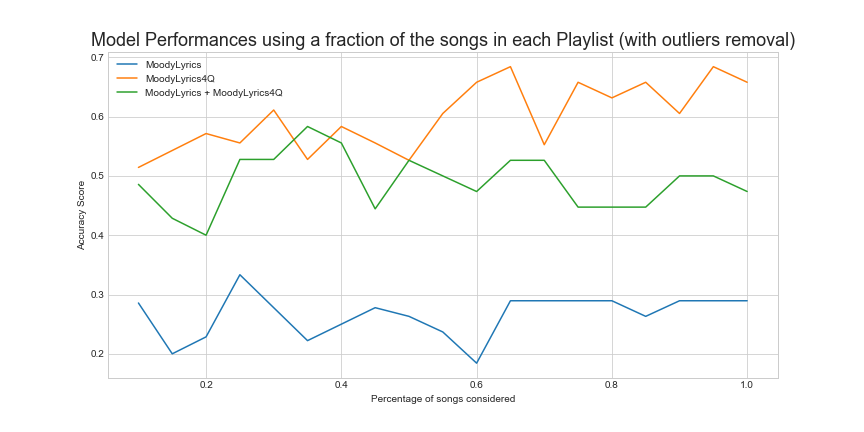
\includegraphics[width=0.9\textwidth]{./chapters/chapter5/images/subset-percentage-robust}
\caption{Classification accuracy on playlists obtained while using robust classification considering just a percentage sample of the total number of songs}
\label{fig:subset-percentage-robust}
\end{figure}

As we can see from those figures, in order to converge to a stable classification accuracy value, the algorithm always needs at least 35 songs. Therefore we believed that this experiment told us that, the best way to classify our playlists is still to consider all of the songs contained in them.

\subsection{Results}
Table \ref{tab:comparison2} shows the different accuracies reached classifying the playlist emotions using the method previously explained. 

\begin{table}[H]
\centering
\begin{tabular}{ |p{3cm}||p{1.5cm}|p{1.5cm}| }
 \hline
 \multicolumn{3}{|c|}{Playlist Classification Accuracy} \\
 \hline
Dataset & With outliers & Without outliers\\
 \hline
MoodyLyrics & 29\% & 29\%\\
MoodyLyrics4Q  & 66\%    &66\%\\
Both together &   50\%  & 47\%\\
\hline
\end{tabular}
\caption{Playlist classification accuracies comparison} \label{tab:comparison2}
\end{table}

\section{Emotion patterns in playlists}
In order to visualize emotion patterns inside a playlist we will use the Silver standard previously created, in which playlists are already classified. We will instead classify the emotion of each song inside a playlist and count the transitions between the emotions.\par
We will use a (4x4) matrix, where $matrix[i][j]$ is the total count of transition from emotion $i$ to emotion $j$ in that playlist. We count a transition from emotion $i$ to emotion $j$ only if the two songs are really consecutive, i.e. if the sequence IDs are consecutive inside the playlist. Indeed since sometimes we cannot download lyrics for a song inside a playlist it is possible that two songs are not really consecutive. \par

In the following figures we show emotion patterns obtained for 2 angry, 2 happy, 2 relaxed and 2 sad playlists. 

\begin{figure}[H]
  \centering
  \begin{subfigure}[b]{0.49\linewidth}
    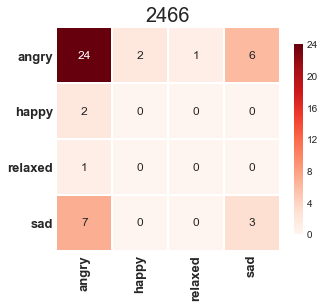
\includegraphics[width=\linewidth]{./chapters/chapter5/images/2466.png}
    \caption{Playlist PID 2466}
  \end{subfigure}
  \begin{subfigure}[b]{0.49\linewidth}
   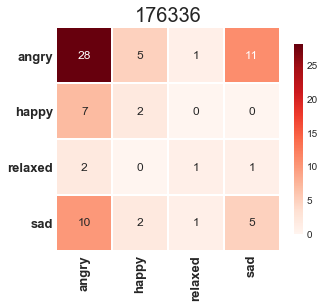
\includegraphics[width=\linewidth]{./chapters/chapter5/images/176336.png}
    \caption{Playlist PID 176336}
  \end{subfigure}
  \caption{Emotion patterns in angry playlists}
  \label{fig:pattern1}
\end{figure}

\begin{figure}[H]
  \centering
  \begin{subfigure}[b]{0.49\linewidth}
    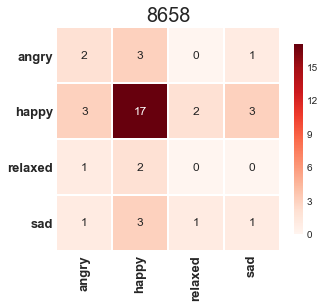
\includegraphics[width=\linewidth]{./chapters/chapter5/images/8658.png}
    \caption{Playlist PID 8658}
  \end{subfigure}
  \begin{subfigure}[b]{0.49\linewidth}
   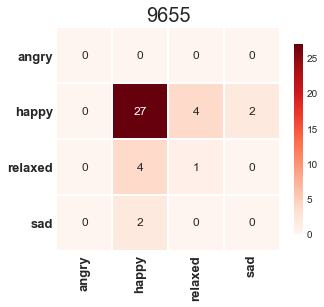
\includegraphics[width=\linewidth]{./chapters/chapter5/images/9655.png}
    \caption{Playlist PID 9655}
  \end{subfigure}
  \caption{Emotion patterns in happy playlists}
  \label{fig:pattern2}
\end{figure}

\begin{figure}[H]
  \centering
  \begin{subfigure}[b]{0.49\linewidth}
    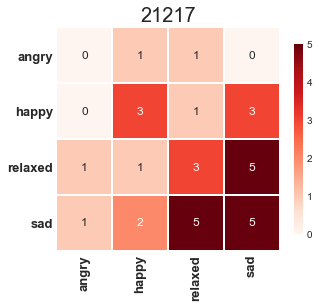
\includegraphics[width=\linewidth]{./chapters/chapter5/images/21217.png}
    \caption{Playlist PID 21217}
  \end{subfigure}
  \begin{subfigure}[b]{0.49\linewidth}
   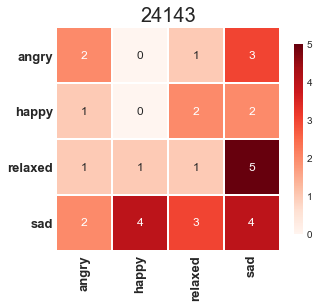
\includegraphics[width=\linewidth]{./chapters/chapter5/images/24143.png}
    \caption{Playlist PID 24143}
  \end{subfigure}
  \caption{Emotion patterns in relaxed playlists}
  \label{fig:pattern3}
\end{figure}

\begin{figure}[H]
  \centering
  \begin{subfigure}[b]{0.49\linewidth}
    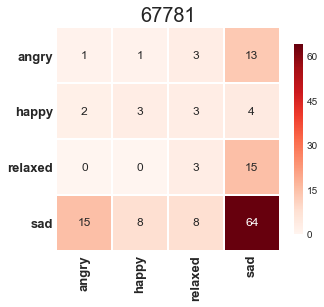
\includegraphics[width=\linewidth]{./chapters/chapter5/images/67781.png}
    \caption{Playlist PID 67781}
  \end{subfigure}
  \begin{subfigure}[b]{0.49\linewidth}
   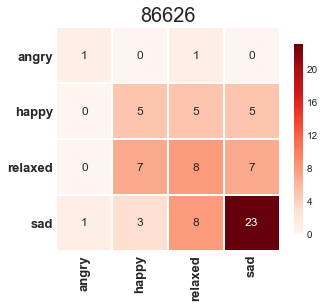
\includegraphics[width=\linewidth]{./chapters/chapter5/images/86626.png}
    \caption{Playlist PID 86626}
  \end{subfigure}
  \caption{Emotion patterns in sad playlists}
  \label{fig:pattern4}
\end{figure}

We can notice that in most of the cases, the greatest number of transitions represents the transition from and to the playlist emotion itself. For example in \textit{angry} playlists not only $matrix[0][0]$ has the biggest count  but also the entire first row and column have the most populated cells, meaning that the majority of times pass from \textit{angry} to \textit{angry} or from \textit{happy}, \textit{relaxed}, \textit{sad} to \textit{angry}. \par

However the \textit{relaxed} playlists represent a more random emotion pattern, meaning that or emotion songs (especially relaxed songs) are badly classified,  or simply relaxed playlist includes a more uniform variety of songs. \par













\begin{thebibliography}{9}
\bibitem{survey} 
Walaa Medhat, Ahmed Hassan, and Hoda Korashy. \textit{Sentiment Analysis Algorithms and Applications: A Survey}. Ain Shams Engineering Journal, 1994.
 
\bibitem{edfromtext} 
Shiv Naresh Shivhare1 and Prof. Saritha Khethawat. \textit{Emotion Detection From Text}, 2012.

 
\bibitem{microsoft} 
Emotion detection and recognition from text using Deep Learning,
\\\href{https://www.microsoft.com/developerblog/2015/11/29/emotion-detection-and-recognition-from-text-using-deep-learning/}{link}

 
\bibitem{ibm_watson} 
IBM Watson: Natural Language Understanding APIs
\\\footnotesize \url{https://www.ibm.com/watson/services/natural-language-understanding/}

\bibitem{ibm_watson_tone} 
IBM Watson: Tone Analyzer
\\\footnotesize \url{https://www.ibm.com/watson/services/tone-analyzer/}

\bibitem{qemotion} 
QEmotion
\\\footnotesize \url{http://www.qemotion.com/demo.php}

\bibitem{moodylyrics} 
MoodyLyrics: A Sentiment Annotated Lyrics Dataset
\\\footnotesize \url{https://www.researchgate.net/publication/317031495_MoodyLyrics_A_Sentiment_Annotated_Lyrics_Dataset}

\bibitem{emoint} 
Shared Task on Emotion Intensity (EmoInt)
\\\footnotesize \url{http://saifmohammad.com/WebPages/EmotionIntensity-SharedTask.html}

\bibitem{emobank} 
EmoBank
\\\footnotesize \url{https://github.com/JULIELab/EmoBank}

\bibitem{features}
Fell, Michael and Caroline Sporleder. "Lyrics-based Analysis and Classification of Music." COLING (2014).

\bibitem{spacy}
SpaCy - Industrial-Strength Natural Language Processing in Python
\\\footnotesize \url{https://spacy.io/}

\bibitem{word2vec}
word2vec - Tool for computing continuous distributed representations of words
\\\footnotesize \url{https://code.google.com/archive/p/word2vec/}

\bibitem{textblob}
TextBlob: Simplified Text Processing
\\\footnotesize \url{http://textblob.readthedocs.io/en/dev/index.html}

\end{thebibliography}
 

\end{document}
              